\section{Problem 9}

\subsection{Instruction}

Use the generateLfsrSequence function you wrote for Problem Set 2 and your
lecture notes to answer the questions.

Which of the following characteristic polynomials correspond to maximal length
sequences for a 9-stage linear feedback shift register? Of those that do, which
pairs of polynomials correspond to so-called preferred pairs of m-sequences,
i.e., m-sequences that can be shifted and summed (modulo 2) to generate a
family of Gold codes?

\subsection{MATLAB code}

\begin{lstlisting}
function [lfsrSeq] = generateLfsrSequence(n,ciVec,a0Vec)
%
% Generate a 1/0-valued linear feedback shift register (LFSR) sequence.
%
% INPUTS
%
% n ------ Number of stages in the linear feedback shift register.
%
% ciVec -- Nc-by-1 vector whose elements give the indices of the Nc nonzero
%          connection elements. For example, if the characteristic polynomial
%          of an LFSR is f(D) = 1 + D^2 + D^3, then ciVec = [2,3] or [3,2].
%
% a0Vec -- n-by-1 1/0-valued initial state of the LFSR, where a0Vec = [a(-1),
%          a(-2), ..., a(-n)]. In defining the initial LFSR state, a
%          Fibonacci LFSR implementation is assumed.
%
% OUTPUTS
%
% lfsrSeq -- m-by-1 vector whose elements are the 1/0-valued LFSR sequence
%            corresponding to n, ciVec, and a0Vec, where m = 2^n - 1. If the
%            sequence is a maximal-length sequence, then there is no
%            repetition in the m sequence elements.

%------------------- FIBONACCI CONFIGURATION ------------------------------

aVec = a0Vec;

m = 0;
lfsrSeq = [];
while (m < 2^n - 1)
    output = aVec(n);
    ai   = mod( sum(aVec(ciVec)), 2);
    aVec = [ai; aVec(1:end-1)] % Allows to see the state (I only care about 
                               % the last one). I prefer not to alter the 
                               % signature of the function.

    lfsrSeq = [lfsrSeq; output];
    m = m+1;
end

end
\end{lstlisting}

\begin{lstlisting}

%% Extra Problem
clc, close all, clear all
%----- Setup
nStages = 9;                 % Number of stages in LFSR

% f1 (D) =1 + D4 + D9
% f2 (D) =1 + D3 + D5 + D6 + D9
% f3 (D) =1 + D3 + D5 + D8 + D9
% f4 (D) =1 + D3 + D4 + D6 + D9
% f5 (D) =1 + D3 + D7 + D8 + D9
% f6 (D) =1 + D2 + D9
ciVec1 = [9, 4]';  
ciVec2 = [9, 6, 5, 3]';
ciVec3 = [9, 8, 5, 3]';
ciVec4 = [9, 6, 4, 3]';
ciVec5 = [9, 8. 7. 3]';
ciVec6 = [9, 2]';

a0Vec1 = ones(nStages,1);

% Examine the final state to determine if it matches the initial and 
% thus conclude that it's indeed a maximal length LFSR
X1 = generateLfsrSequence(nStages,ciVec1,a0Vec1); % maximal length
X2 = generateLfsrSequence(nStages,ciVec2,a0Vec1); % maximal length
X3 = generateLfsrSequence(nStages,ciVec3,a0Vec1); % not maximal lenght
X4 = generateLfsrSequence(nStages,ciVec4,a0Vec1); % maximal length
X5 = generateLfsrSequence(nStages,ciVec5,a0Vec1); % not maximal length
X6 = generateLfsrSequence(nStages,ciVec6,a0Vec1); % not maximal length

% Now let's see if it's a Gold sequence by analizing the cross-correlation

%----- Compute crosscorrelation 
[R12,iiVec] = ccorr(X1,X2);
[R13,iiVec] = ccorr(X1,X3);
[R23,iiVec] = ccorr(X2,X3);

figure()
subplot(1,3,1)
plot(R12)
title('R12')
grid on

subplot(1,3,2)
plot(R13)
title('R13')
grid on

subplot(1,3,3)
plot(R23)
title('R23')
grid on
\end{lstlisting}

\subsection{Results}

To determine if the characteristic polynomials correspond to maximal length
sequences for a 9-stage ($n=9$) LFSR one needs to check if the state of the LFSR
($a_i$) is the same as the initial state after generating a sequence of
length $N=2^n -1$. As indicated in the MATLAB code, the characteristic polynomials
1, 2 and 4 correspond to maximal length sequence generators.

The characteristic of the Gold sequences is that their cross-correlation is
defined by the following

\begin{equation}
	R_{ab}(k) = { -t(n), -1, t(n) - 2}
\end{equation}

Where $t(n) = 1 + 2^{(n+1)/2}$ if n is odd. And $t(n) = 1 + 2^{(n+2)/2}$ if n is
even. So, you have a guarantee that the cross-correlation is bounded. In our case,
n=9. Then the $|R_ab(k)| < 33$. The autocorrelation follows a similar pattern
as the cross-correlation except at the main peak. Figure~\ref{fig:ex9_crosscorr}
shows the cross-correlation for all the maximal-length sequences pairs. The
conclusion is that the sequences are not Golden since neither respect the bound.

\begin{figure}[H]
	\centering
	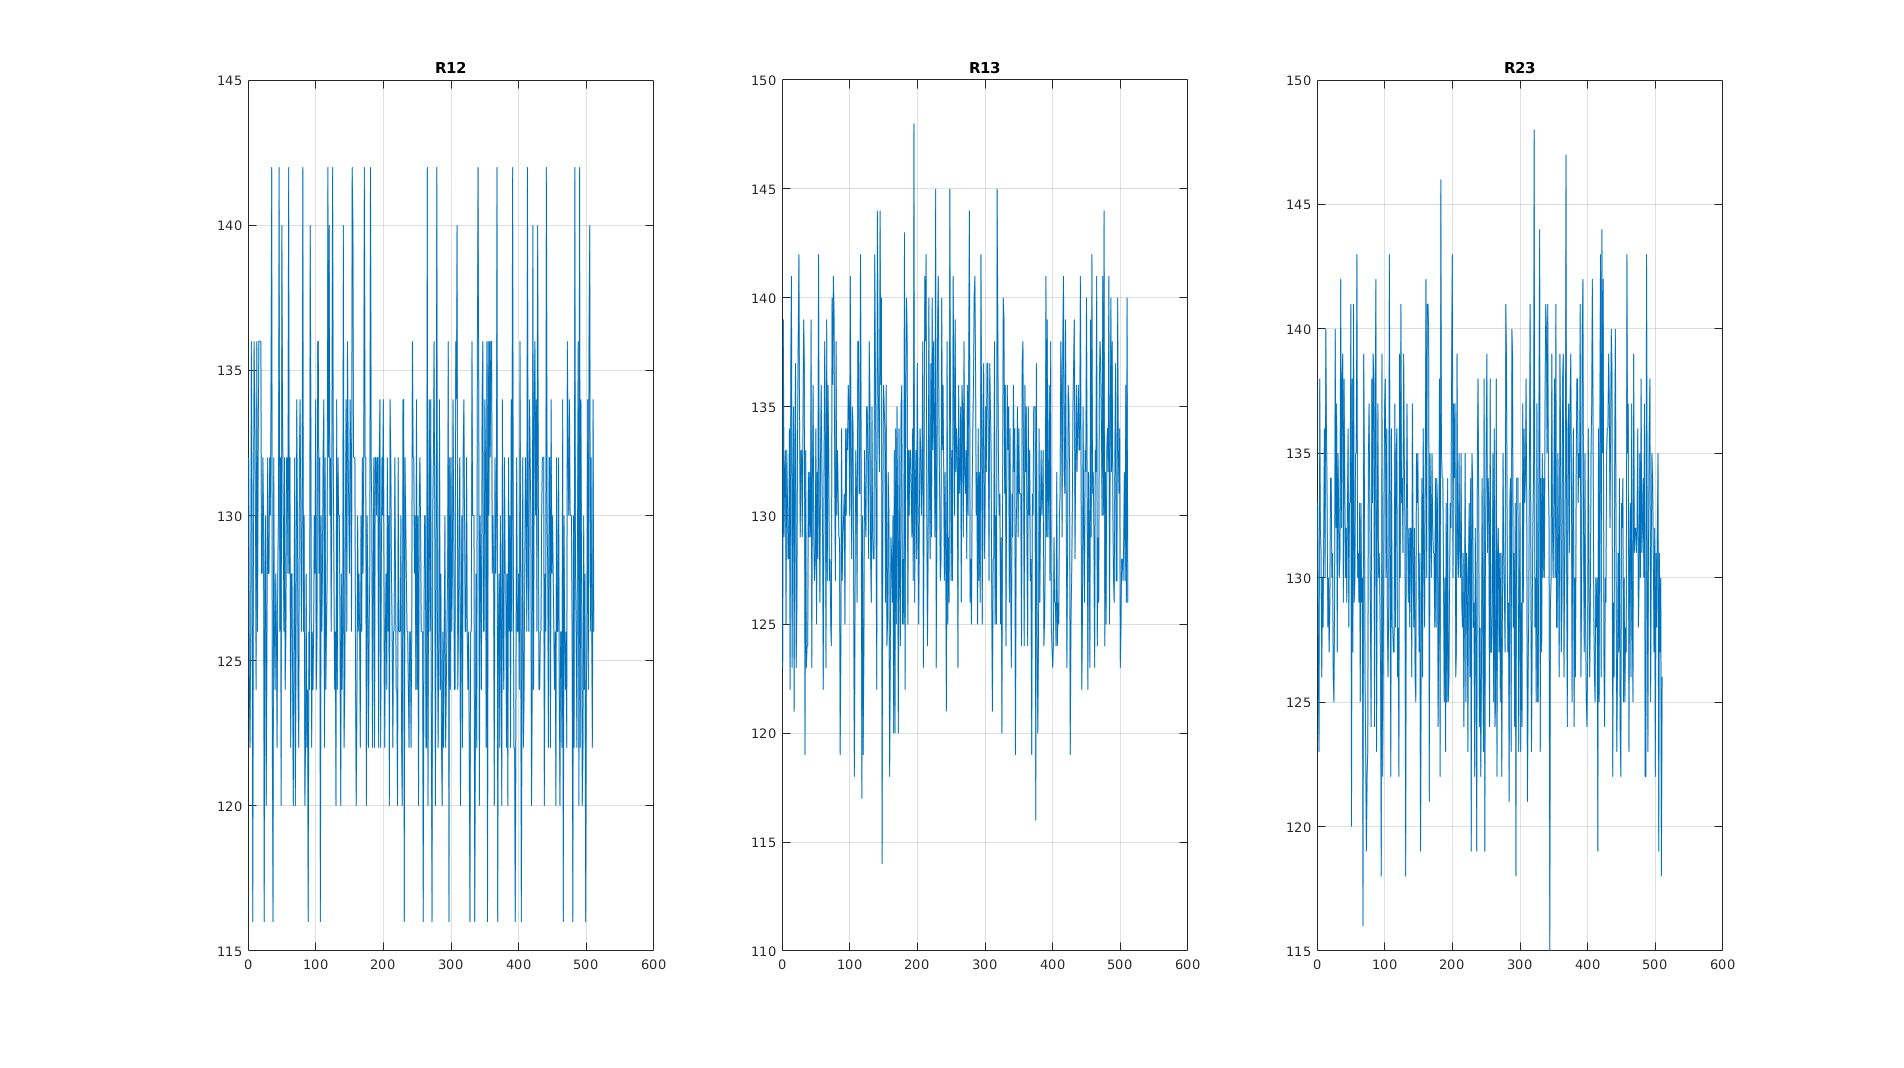
\includegraphics[width=0.9\textwidth]{figs/ex9_crosscorr.png}
	\caption{Cross-correlation of all the maximal length sequences.}
	\label{fig:ex9_crosscorr}
\end{figure}

